\section{Marco Teórico}

A continuación se presentan las variables que consideramos importantes para el desarrollo del proyecto, antes de llevar a cabo la elección de los dispositivos a emplear, previamente se elaboró una investigación de los signos vitales más indispensables del ser humano, por lo que para fines del proyecto y de acuerdo con lo analizado las variables a medir son la temperatura, considerando que es el primer parámetro para determinar una enfermedad, la segunda variable es un acelerómetro que por causa del envejecimiento de las personas suelen ser más predispuestas a sufrir alguna caída y por último la frecuencia cardíaca, esta última involucra un órgano muy importante para las personas por ello consideramos evaluar conjuntamente esta medida. Existen otras variables importantes pero por la complejidad para medirlas no entran en la posibilidad de incluirlas en este trabajo terminal, dichas variables pueden ser por ejemplo: la presión arterial, la glucosa, por mencionar algunas, ya que al medirlas no utilizan un método invasivo y no causan molestia al usuario. \\

\subsection{Variables a medir}

En este apartado se muestra una descripción de las variables que elegimos y la importancia de cada una, de igual forma se explicaran los motivos por los que fueron seleccionadas. A continuación se en listan las variables seleccionadas y las cuales serán monitoreadas en este proyecto:

\begin{enumerate}
	\item Temperatura.
	\item Caídas.
	\item Frecuencia Cardíaca.
\end{enumerate}

\begin{enumerate}
	\item \textbf{Temperatura} 
	
	Se ha considero medir la temperatura corporal, está variable es de gran importancia para determinar las condiciones en las que se encuentra el enfermo, la constante medición de esta permite a enfermeros(as) y algún otro personal médico conocer la mejoría y situación del paciente, en algunos casos la temperatura se toma como primer parámetro para diagnosticar una enfermedad. \\
	
	La Secretaria de Salud establece que la temperatura corporal aceptable oscila entre los $36.5^{\circ}$C $47^{\circ}$C y los $37.2^{\circ}$C, mientras que las temperaturas fuera de este rango se consideran anormales, a continuación, se muestran los términos utilizados considerados anormales conforme a la Norma Oficial Mexicana NOM-031-SSA2-1999, considerando que no interviene un mecanismo termorregulador o se presenta un golpe de calor.
	
	\begin{itemize}
		\item \textbf{Fiebre:} La elevación anormal de la temperatura corporal por encima de los $38^{\circ}$C.
		\item \textbf{Hipertermia:} Es el estado de incremento de la temperatura del cuerpo que sobrepasa los $40^{\circ}$C.
		\item \textbf{Hipotermia:} En este estado la temperatura corporal se encuentra por debajo de los $36^{\circ}$C.
	\end{itemize}
	
	Por esta razón es importante tener controlada la temperatura en el rango que se considera aceptable. Nuestro cuerpo tiene mecanismos que regulan la temperatura y con el paso de los años se van perdiendo. Por esta importancia se decidió tomar la temperatura como una de las variables a medir en este proyecto \cite{once}.
	
	\item \textbf{Caídas}
	
	Las caídas son consideradas de alta importancia, debido las consecuencias que conllevan y pueden sufrir las personas de la tercera edad. Los tipos de caídas en adultos mayores pueden ser las siguientes:
	
	\begin{itemize}
		\item \textbf{Caída accidental:} Es aquella que generalmente se produce por una causa ajena al adulto mayor sano (ejemplo: tropiezo) y que no vuelve a repetirse.
		\item \textbf{Caída repetida:} Expresa la persistencia de factores predisponentes como, enfermedades crónicas múltiples, fármacos, pérdidas sensoriales, etc.
		\item \textbf{Caída prolongada:} Es aquella en la que el adulto mayor permanece en el suelo por más de 15 o 20 minutos por incapacidad de levantarse sin ayuda.	Los adultos mayores que tienen mayor prevalencia de caídas prolongadas son: aquellos de 80 años o más, con debilidad de miembros, con dificultades para las actividades cotidianas y aquellos que toman medicación \cite{doce}.
	\end{itemize}

	\begin{itemize}
		\item Escenarios y posturas de una persona al sufrir una caída.
		Para entender los escenarios y posturas se realizó un estudio con 240 personas de la tercera edad para monitorear sus actividades cotidianas (como: sentarse en una silla, sentarse en un inodoro, salir o entrar de un auto, sentarse o recostarse sobre la cama y caminar), a estas personas se les coloca un acelerómetro en diferentes partes del cuerpo, el cual detecta las señales tanto de las actividades mencionadas, como de alguna caída (caídas hacia delante o atrás, caídas laterales a la izquierda o derecha y caídas con las piernas rectas o flexionadas) que lleguen a sufrir los sujetos de estudio \cite{trece}. \\
		 
		En la figura 1.3 se detectaron los umbrales superior e inferior de caídas, donde se observa que estas tienen una señal con un pico muy alargado el cual está en un rango de aceleración de entre 0 y 7 g, a diferencia de la señal de las actividades cotidianas que no rebasan 1.5 g. \\
		
		\begin{figure}[h]
			\centering
			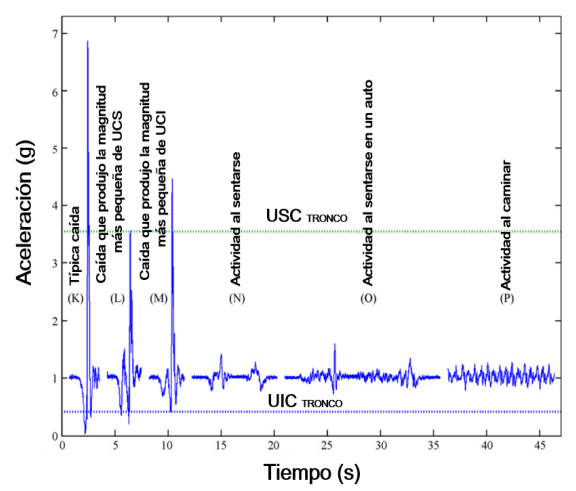
\includegraphics[scale=0.35]{introduccion/imagenes/grafica1_3}
			\textbf{\caption{\small{Representación de una señal para caídas y actividades cotidianas, en personas de la tercera edad usando un acelerómetro \cite{trece}.}}}
			\label{Seccion1.5.1:Figura1.3}
		\end{figure}
		
		En la figura 1.4 se muestran detalladamente los puntos de interés en la señal y cada una de las posiciones en las que se encontraba el adulto mayor al sufrir una caída, de igual manera se muestran detalladamente las actividades cotidianas realizadas en donde el acelerómetro registro actividad con pequeñas variaciones y similitudes, mostrando los puntos de interés en dicha señal.  \\
		
		\begin{figure}[h]
			\centering
			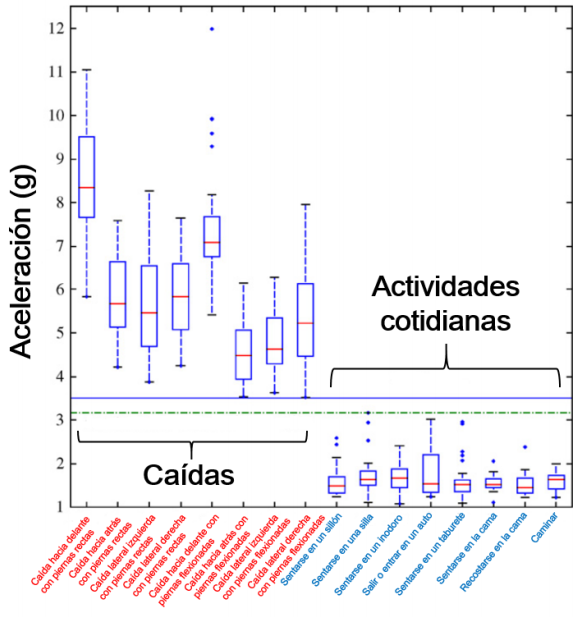
\includegraphics[scale=0.35]{introduccion/imagenes/grafica1_4}
			\textbf{\caption{\small{Puntos de interés en la señal que muestra: (a) posturas al sufrir una caída y (b) actividades cotidianas \cite{trece}.}}}
			\label{Seccion1.5.1:Figura1.4}
		\end{figure}
		
		Con base en las figuras 1.3 y 1.4 se establecen los escenarios en los que una persona puede sufrir algún tipo de caída y en donde se utilizan sensores acelerómetros en diferentes partes del cuerpo para realizar un muestreo de la aceleración. \\
		
		\begin{table}
%			\centering
			\resizebox*{12.5cm}{8cm}{
				\begin{tabular}{|l|c|c|c|}
					\hline
					Escenario & Postura	& Muestreo del acelerómetro & Caída \\
					\hline \hline
					Caída hacia adelante con piernas rectas	& De pie o recostado & 7.5g a 9.5g & Si \\
					\hline
					Caída hacia atrás con piernas rectas & De pie o recostado & 5g a 6.5g & Si \\
					\hline
					Caída lateral izquierda con piernas rectas & De pie o recostado & 4.5g a 6.5g & Si \\
					\hline
					Caída lateral derecha con piernas rectas & De pie o recostado & 5g a 6.5g & Si \\
					\hline
					Caída hacia adelante con piernas flexionadas & Sentado o inclinado & 6.8g a 7.8g & Si \\
					\hline
					Caída hacia atrás con piernas flexionadas & Sentado o inclinado & 4g a 5g & Si \\
					\hline
					Caída lateral izquierda con piernas flexionadas & Sentado o inclinado & 4.5g a 5.5g & Si \\
					\hline
					Caída lateral derecha con piernas flexionadas & Sentado o inclinado & 4.8g a 6g	& Si \\
					\hline
					Sentarse en un sillón & Sentado	& 1.2g a 1.8g & No \\
					\hline
					Sentarse en una silla & Sentado & 1.5g a 1.9g &	No \\
					\hline
					Sentarse en un inodoro & Sentado & 1.5g a 2g & No \\
					\hline
					Salir o entrar de un auto & Sentado o de pie & 1.2g a 2.5g & No \\
					\hline
					Sentarse en un taburete & Sentado & 1.2g a 1.5g & No \\
					\hline
					Sentarse en la cama	& Sentado & 1.4g a 1.6g & No \\
					\hline
					Recostarse en la cama & Recostado & 1.2g a 1.6g & No \\
					\hline
					Caminar & De pie & 1.5g a 1.8 & No \\
					\hline
				\end{tabular}
			}
		\textbf{\caption{\small{\textbf{Escenarios y posturas en los que el acelerómetro realizará muestreo.}}}}
		\end{table}
	
	 Por lo anterior y debido a la complejidad de detectar todos los escenarios de caídas, en este proyecto únicamente se detectará la caída típica, que es la caída hacia delante con las piernas rectas.
	\end{itemize}

	\item \textbf{Frecuencia Cardíaca}
	
	Esta variable es considerada importante puesto que involucra uno de los signos más relevantes para el óptimo funcionamiento del corazón, de modo que es el principal órgano del ser humano que nos mantiene con vida, por lo cual estimaremos dicha variable para este proyecto. \\
	
	El funcionamiento del corazón se manifiesta, al actuar como bomba impulsora, lo que determina el gasto cardíaco (cantidad de sangre enviada por el corazón al torrente circulatorio en un minuto), que representa el volumen de eyección sistólico en cada latido por minuto. La frecuencia cardíaca (FC) es un parámetro indicativo de la eficiencia con la que el corazón trabaja. En esfuerzos de tipo máximo se busca alcanzar la frecuencia cardíaca máxima para cada sujeto, sin pasar los límites que representen riesgo de provocar una falla o insuficiencia cardíaca durante la ejecución de un esfuerzo físico intenso. Para determinarla existen varios modelos matemáticos, pero el más común consiste en tomar la cifra de 220 y restarle la edad del sujeto. \\
	
	Por otro lado, habitualmente la tensión arterial se incrementa con la edad, más la sistólica que la diastólica, así como la presión del pulso (diferencia entre ambas), en las personas mayores de 65 años, el 40\% sufre de hipertensión arterial, y de ellos el 65\% - 70\% tienen riesgo de sufrir accidentes cardiovasculares, fatales o no. \\
	
	Con el paso de los años, el organismo pierde su habilidad para redistribuir el flujo sanguíneo desde las vísceras a los músculos en acción, de tal forma que la diferencia arteriovenosa de oxígeno (Dif a/v O2) medida en el músculo y la del flujo de retorno venoso al corazón durante el esfuerzo físico, es menor en las personas adultas mayores y sedentarias, con lo cual disminuye la reserva funcional \cite{catorce}. \\
	
	Algunos estudios realizados en poblaciones sanas, así como en pacientes hipertensos, con cardiopatía isquémica o con insuficiencia cardíaca, demuestran una asociación entre la FC elevada y un mayor riesgo de mortalidad. Según esto, cuanto mayor es la FC, menor es la expectativa de vida. La frecuencia cardíaca (FC) en reposo oscila entre 50 y 100 latidos por minuto en las personas adultas. Al nacer, la FC es más elevada porque el bebé la necesita para su adecuado crecimiento. A partir del primer mes de vida, la FC va disminuyendo hasta alcanzar las cifras normales de un adulto. El ejercicio físico o las situaciones de estrés provocan un aumento de la FC (taquicardia sinusal), que se considera normal \cite{quince}.
	
\end{enumerate}

\subsection{Sensores}

A continuación, se muestran algunas definiciones de la investigación de los sensores que ayudaran a la realización de este proyecto. \\

Un dispositivo electrónico que produce datos eléctricos, ópticos o digitales derivadas de una condición física o evento. La Real Academia Española lo define como un dispositivo que detecta una determinada acción externa y es transmitida adecuadamente. \\

Conociendo estas definiciones llamaremos sensor al dispositivo o mecanismo eléctrico que nos permite medir una variable física, dando como respuesta una señal o dato en relación con la magnitud de la variable medida. \\

\subsection{Sensor de temperatura}

\textbf{Definición} \\

Es un dispositivo que permite medir los cambios de la temperatura y entregar una señal eléctrica en relación a la magnitud de la temperatura. Son usados para asegurar que la temperatura de un proceso esté en su normalidad o bien tener la temperatura en un rango especificado siendo obligatorio cumplir con la condición. \\

La variedad de sensores de temperatura está relacionada con el material del que están hechos, del uso que se les pretenda dar en función con las temperaturas que soporten y como es que responden a la magnitud medida, estas respuestas pueden ser en voltaje, resistencia, corriente y señales digitales. \\

Entre los más utilizados se encuentran los termistores NTC (Coeficiente de Temperatura Negativa) y PTC (coeficiente de temperatura Positiva), termopares, RTD (Detectores de Temperatura por Resistencia), circuitos integrados y detectores de temperatura por luz infrarroja. \\


\begin{figure}[h]
	\centering
	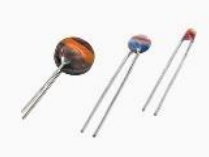
\includegraphics[scale=0.35]{introduccion/imagenes/termistores}
	\textbf{\caption{\small{Termistores \cite{dieciseis}.}}}
	\label{Seccion1.5.1:Figura1.5}
\end{figure}

\textbf{Tipos de sensores de temperatura} \\

\textbf{RTD} \\

Los RTD son sensores de temperatura que utilizan la propiedad de resistencia y coeficiente térmico de un metal (conductor), se basan en el principio de equilibrio térmico que señala que cuando un metal se encuentra en un medio que tiene mayor temperatura que él, éste tiende a aumentar su temperatura, siempre y cuando el volumen y la masa no sean mayor que el del medio con el que interactúa. Las RTD son utilizadas en el sector industrial, entre las características más destacadas es su resistencia a altas temperaturas, su alta sensibilidad, tienen una exactitud mínima de $1^{\circ}$C, tienen un tiempo de vida alto. \\

\textbf{NTC} \\

Las NTC son sensores elaborados por óxidos semiconductores que responden disminuyendo su resistencia a medida que aumenta la temperatura, son sensores con alta sensibilidad, son utilizados para monitorear que la temperatura no sobrepase un rango. \\

\textbf{PTC} \\

Las PTC son termistores con un coeficiente de temperatura positivo que al aumentar la temperatura aumenta su resistencia, son elaborados con óxidos y conductores, se utilizan para elaborar sistemas de control de temperatura, con el fin de no sobrepasar cierta temperatura ya que esta puede ser critica \cite{diecisiete}. \\

\textbf{Termopares} \\

Son sensores que se elaboran uniendo dos conductores, están basados en el principio de Seebeck y Peltier, el efecto de Seebeck dice que cuando la unión de los metales presenta diferentes temperaturas se produce un voltaje muy pequeño, que va en incremento con la temperatura, mientras que el efecto Peltier dice que transmitir una corriente en la unión de los metales se produce un flujo de calor. Los termopares se utilizan en sistemas de refrigeración para disminuir las temperaturas o aumentarlas, además de sensar la temperatura \cite{dieciocho}. \\

\textbf{Sensores a base de Circuitos Integrados} \\

Los circuitos integrados son dispositivos que están formados de elementos electrónicos, que permiten tener la misma funcionalidad que un circuito electrónico, solo que en un espacio reducido. En la actualidad tienen funciones específicas desde reguladores de voltaje, corriente hasta medir temperatura. \\

\textbf{Sensores Infrarrojos} \\

Otra de las propuestas interesantes que tenemos son los sensores de radiación térmica, estos funcionan midiendo la energía que emiten los objetos, en la región infrarroja, están construidos por un sistema óptico que enfoca el objeto, utilizando un diodo láser que ilumina la zona captando la energía desprendida de los objetos. \\

Presentan un inconveniente acorde a los materiales que presentan emisividad, que es la proporción de radiación térmica emitida por una superficie u objeto debido a su temperatura. \\

Los cuerpos negros presentan una emisividad igual a uno, en la práctica todos los cuerpos tienen esta propiedad de acuerdo a su color, los sensores de radiación vienen ajustados para una emisividad predeterminada, por lo que si se tiene otra emisividad diferente se tendrá que calibrar \cite{diecinueve}. \\










